% !TEX root = Projektdokumentation.tex
\section{Anhang}

\subsection{Detaillierte Zeitplanung}
\label{app:Zeitplanung}
\tabelleAnhang{ZeitplanungKomplett}

\clearpage
\subsection{Klassendiagramm}
\label{app:Klassendiagramm}

Die grün umrandeten Klassen sind verwendete, bereits existierende Klassen der Code-Basis.
Alle schwarz umrandeten Klassen sind durch dieses Projekt entstanden.

\begin{figure}[htb]
\centering
\includegraphicsKeepAspectRatio{Klassendiagramm.png}{1.2}
\caption{Vollständiges Klassendiagramm}
\end{figure}

\subsection{Sequenzdiagramm}
\label{app:Sequenzdiagramm}

\begin{figure}[htb]
	\centering
	\includegraphicsKeepAspectRatio{Sequenzdiagramm.png}{1}
	\caption{Sequenzdiagramm}
\end{figure}

\clearpage
\subsection{Screenshots der Anwendung}
\label{app:Screenshots}

\begin{figure}[htb]
	\centering
	\includegraphicsKeepAspectRatio{Dokumentenbaum.png}{0.7}
	\caption{Dokumentenbaum mit den verschiedenen Dokumenttypen sortiert nach Prüfgebieten}
\end{figure}

\begin{figure}[htb]
	\centering
	\includegraphicsKeepAspectRatio{Menueeintrag.png}{0.7}
	\caption{Menüeintrag zum Anstoß des Globalen Aktualisierens}
\end{figure}


\clearpage
\subsection{Testfälle}
\label{app:Test}

\begin{figure}[htb]
	\centering
	\includegraphicsKeepAspectRatio{UnitTest.png}{1}
	\caption{Komponententest}
\end{figure}

%\lstinputlisting[language=php]{Listings/tests.php}
%\clearpage
%\begin{figure}[htb]
%\centering
%\includegraphicsKeepAspectRatio{testcase.jpg}{1}
%\caption{Aufruf des Testfalls auf der Konsole}
%\end{figure}

%\subsection{Entwicklerdokumentation}
\label{app:Doc}

\gqq{hier könnte ihre Entwicklerdokumentation stehen}

%\begin{center}
%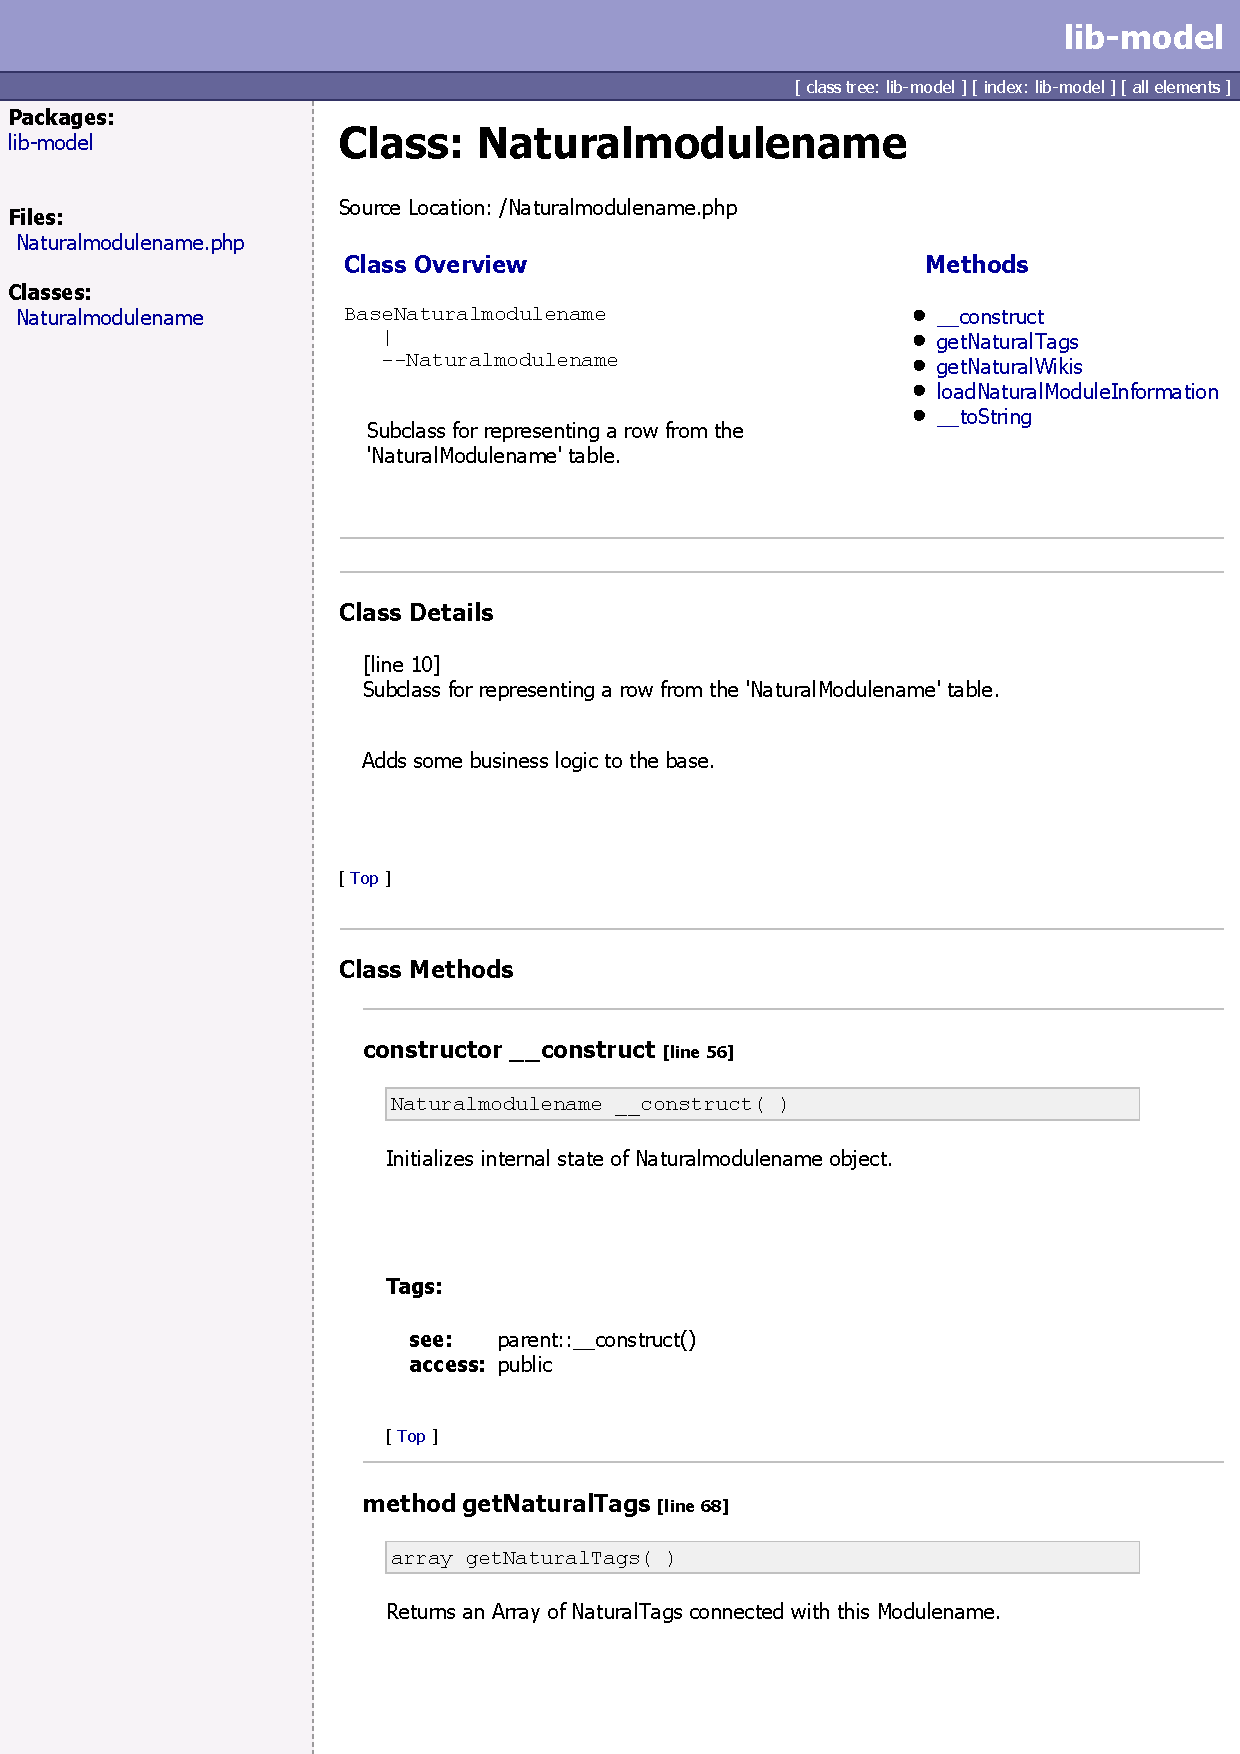
\includegraphics[page=1, width=0.9\textwidth]{doc.pdf}
%
%\includegraphics[page=2, width=0.9\textwidth]{doc.pdf}
%\end{center}

%\subsection{Benutzerdokumentation}
\label{app:BenutzerDoku}
Ausschnitt aus der Benutzerdokumentation:

\gqq{hier könnte ihre Benutzerdokumentation stehen}

%\begin{table}[htb]
%\begin{tabularx}{\textwidth}{cXX}
%\rowcolor{heading}\textbf{Symbol} & \textbf{Bedeutung global} & \textbf{Bedeutung einzeln} \\
%\includegraphicstotab[]{weather-clear.png} & Alle Module weisen den gleichen Stand auf. & Das Modul ist auf dem gleichen Stand wie das Modul auf der vorherigen Umgebung. \\
%\rowcolor{odd}\includegraphicstotab[]{weather-clear-night.png} & Es existieren keine Module (fachlich nicht möglich). & Weder auf der aktuellen noch auf der vorherigen Umgebung sind Module angelegt. Es kann also auch nichts übertragen werden. \\
%\includegraphicstotab[]{weather-few-clouds-night.png} & Ein Modul muss durch das Übertragen von der vorherigen Umgebung erstellt werden. & Das Modul der vorherigen Umgebung kann übertragen werden, auf dieser Umgebung ist noch kein Modul vorhanden. \\
%\rowcolor{odd}\includegraphicstotab[]{weather-few-clouds.png} & Auf einer vorherigen Umgebung gibt es ein Modul, welches übertragen werden kann, um das nächste zu aktualisieren. & Das Modul der vorherigen Umgebung kann übertragen werden um dieses zu aktualisieren. \\
%\includegraphicstotab[]{weather-storm.png} & Ein Modul auf einer Umgebung wurde entgegen des Entwicklungsprozesses gespeichert. & Das aktuelle Modul ist neuer als das Modul auf der vorherigen Umgebung oder die vorherige Umgebung wurde übersprungen. \\
%\end{tabularx}
%\end{table}


